% 
% PARTIE 1
% 
\section{Contexte et présentation du système}
\subsection{Contexte}



Les éruptions volcaniques peuvent avoir un impact important sur l'activité humaine, provoquant à
la fois des déplacements de population, des dégâts matériels, ainsi que des changements de
topographie et de climat. On considère qu'actuellement 10\% de la population terrestre vit sous la
menace des volcans, et 1500 volcans potentiellement en activité sont répertoriés sur la planète.
Par conséquent, une compréhension fine des phénomènes volcaniques et une meilleure maîtrise
des risques associés constituent un enjeu scientifique majeur.

Les observations scientifiques réalisées pendant les phases éruptives sont aujourd'hui
fondamentales pour l'étude des volcans. En effet, les prélèvements des gaz magmatiques et des
échantillons rocheux rejetés lors de ces phases constituent des indicateurs fiables de l'activité
interne des volcans ; ils sont donc une riche source d'informations pour les volcanologues.
Cependant, les phases éruptives sont aussi des phases actives très dangereuses et il est
primordial de limiter les risques humains lors d'observations et de prélèvements à proximité des
cratères en éruption (\autoref{fig_01}). 



\begin{figure}[H]
\centering
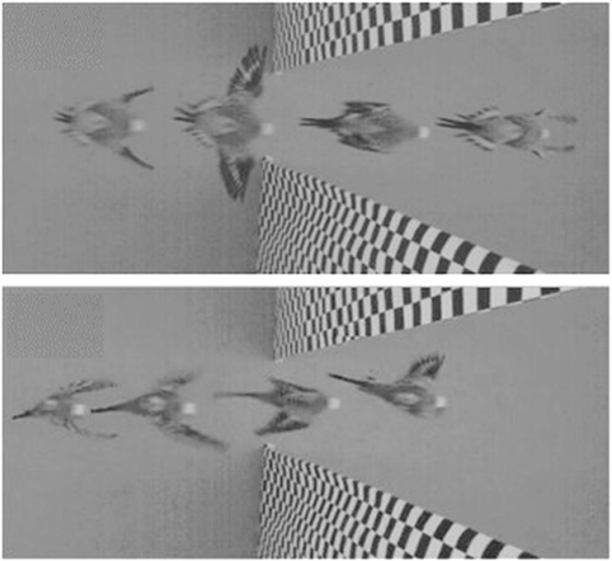
\includegraphics[width=.45\linewidth]{fig_01.png}
\caption{Schématisation d'un volcan en éruption \label{fig_01}}
\end{figure}


Avec ce constat, allié aux avancées technologiques dans le domaine de la robotique, la
Communauté Européenne a financé le projet ROBOVOLC dont le but était la réalisation d'un robot
mobile pour l'exploration volcanique. Ce robot devait être capable de :
\begin{itemize}
\item s'approcher d'un cratère actif ;
\item collecter des échantillons rocheux issus de rejets éruptifs ;
\item collecter des échantillons gazeux ;
\item collecter d'autres données physiques et chimiques.
\end{itemize}


\begin{obj}
Le sujet propose d'étudier quelques parties structurelles du système ROBOVOLC et de
valider plusieurs performances (liées à la mobilité et au prélèvement) de ce système. 
\end{obj}

\subsection{Présentation du système}


Le système ROBOVOLC est représenté sur la \autoref{fig_02}. Il se divise en plusieurs sous-systèmes
(liés à la navigation, au prélèvement et à la communication) qui sont détaillés dans les
diagrammes SysML fournis dans l'Annexe 1. 

\begin{figure}[H]
\centering
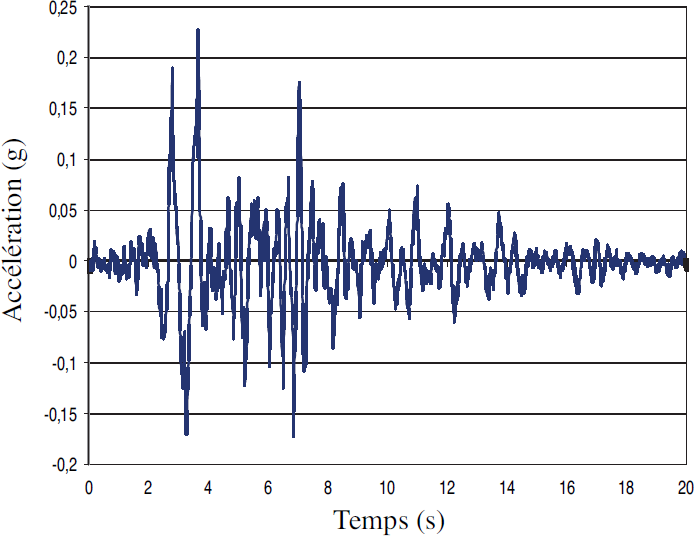
\includegraphics[width=.45\linewidth]{fig_02.png}
\caption{Représentation du système ROBOVOLC \label{fig_02}}
\end{figure}

La partie mécanique de ROBOVOLC est constituée de deux parties : (i) la plateforme (châssis,
roues) servant à la locomotion ; (ii) l'équipement d'analyse (bras manipulateur, pince, sondes) pour
le prélèvement et la mesure.

Une contrainte particulière dans la conception du système ROBOVOLC est qu'il est soumis à des
conditions extérieures particulièrement difficiles : terrain volcanique non structuré avec obstacles et
fortes pentes, températures très élevées près des zones éruptives (les gaz atteignent 600\degres C) mais
basses ailleurs à cause de l'altitude, présence de poussières de cendre très fines, ambiance
corrosive due aux composants acides, etc.


%Q1.1 : 
\question{Dans la phase de conception de ROBOVOLC, une alternative à un système de locomotion
à roues était un système volant. Donner deux inconvénients d'un tel système remettant en cause
son utilisation dans l'environnement volcanique considéré.}

ROBOVOLC est piloté à distance depuis un poste de contrôle (\autoref{fig_03}). La position géographique
du robot est obtenue par un système GPS et est envoyée au poste de contrôle par liaison radio.
De plus, l’opérateur peut visualiser en permanence les actions du système grâce aux images
transmises par une caméra embarquée.

L'énergie électrique nécessaire au système est apportée par une unité de puissance avec quatre
batteries couplées pour constituer deux unités de 24 V. La première est utilisée pour la plateforme,
l'autre pour l'équipement d'analyse. Ces batteries sont positionnées sur la partie basse du châssis.

%Q12
\question{Citer un intérêt à mettre les batteries en position basse sur le système.}


\begin{figure}[H]
\centering
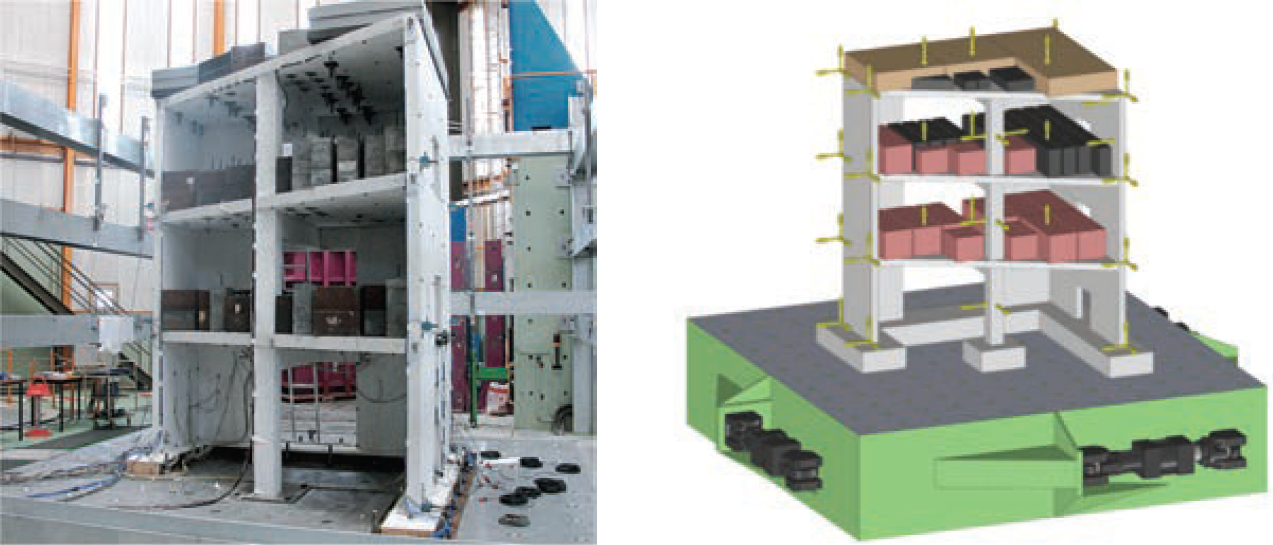
\includegraphics[width=.45\linewidth]{fig_03.png}
\caption{Illustration du pilotage à distance du système ROBOVOLC\label{fig_03}}
\end{figure}

Un cahier des charges partiel est donné ci-dessous :

\begin{center}
\begin{tabular}{ll}
\hline
\textbf{Critère} & \textbf{Valeur} \\ \hline \hline
Distance maximale entre ROBOVOLC et le poste de contrôle & \SI{2}{km} \\ \hline  
Temps de trajet pour une mission de 24 heures 		& \SI{1,5}{h} \\ \hline 
Vitesse de déplacement atteignable 				& \SI{0,5}{m/s} \\ \hline 
Dimensions du système (longueur/largeur/hauteur) 		& \SI{1900}{mm} x \SI{1200}{mm}x \SI{800}{mm}\\ \hline 
Masse maximale des composants modulaires 			& \SI{200}{kg} \\ \hline 
Charge utile maximale (instruments, etc.) 			& \SI{30}{kg} \\ \hline 
Pente maximale du sol 						& 40\degres \\ \hline 
Hauteur maximale d'un obstacle 					& \SI{400}{mm} \\ \hline 
Diamètre des objets à saisir entre 				& \SI{40}{mm} et \SI{300}{mm} \\ \hline 
Masse maximale des objets à saisir 				& \SI{2,5}{kg} \\ \hline 
\end{tabular}
\end{center}



%Q1.3 : 
\question{Citer une phase de vie du système qui contraint sa taille maximale et son poids maximal.}

La suite du sujet est composée de quatre parties qui étudient quelques particularités de la
structure mécanique du système ROBOVOLC :
\begin{itemize}
\item les parties \ref{sec_2} et \ref{sec_3} étudient la phase de déplacement (roulage) du système : la partie \ref{sec_2} vise
à valider les performances de mobilité et de suivi de trajectoire du système sur un sol plan
tandis que la partie \ref{sec_3} vise à valider les performances de franchissement d'obstacle sur un
terrain accidenté ;
\item les parties \ref{sec_4} et \ref{sec_5} étudient la phase de préhension d'échantillon : la partie \ref{sec_4} vise à valider
les performances du bras manipulateur tandis que la partie \ref{sec_5} vise à valider les
performances de la pince.
\end{itemize}


